\documentclass[./../../paper.tex]{subfiles}
\graphicspath{{\subfix{./../../figures/}}}

\begin{document}

\section{Determine the Evolutionary Algorithm Hyperparameter settings}

\subsection{Experimental Setup}
\label{sec:exp2}
Given the combinatory set of configurations chosen in \autoref{sec:exp1}, we will explore optimal parameter setting. Therefore, we run each configuration with a multitude of different hyperparameter settings. 

For each configuration we vary the mutation rates and edit rates. The mutation rates for every edit-type are each between 0 and 1 and sum to 1. For the edit rate we explore values between 0.1 and 0.9. We do not, explore the extremes for the edit-rate as this would amount to either never changing the sequence or completely changing the sequence. An edit-rate of 0 would translate to never changing the sequence. This conflicts with the very core of generating counterfactuals. An edit-rate of 1 amounts to changing the complete sequence, which makes the convergence to an optimum impossible. 

We use the resulting viability and feasibility as dependent variables and each hyperparameter as independent variable.

Furthermore, it confilicts with the Sparcity and Similarity criterions. The remaining procedure follows the process described in \autoref{sec:exp1}.


\subsection{Results}
\attention{Correlation matrix makes no sense. It should be only a bar plot with feasibility and viability with all the hyperparams.}

\begin{figure}
    \centering
    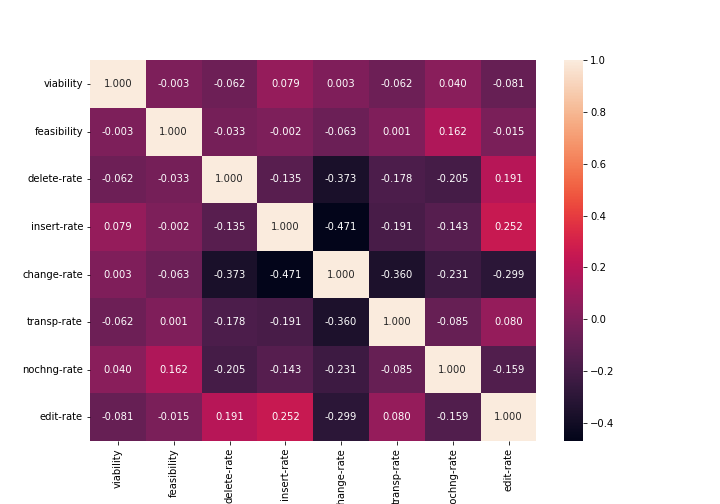
\includegraphics[width=\textwidth]{figures/results/params_heatmap.png}
    \caption{Shows a correlation matrix of each hyperparameter, the feasibility measure and the viability measure.}
    \label{fig:param_results_1}
\end{figure}

\needstbl{tbl:viability_params}{This table shows the results of the mixed linear model using viability as dependent variable.}

\needstbl{tbl:feasibility_params}{This table shows the results of the mixed linear model using feasibility as dependent variable.}

\autoref{fig:param_results_1} suggests that all hyperparamers have a negative correlation with feasibilty and viability. However, if we consider the results of the effects models we see that the interaction of edit-rate with \attention{a couple of hyperparamers} show that some parameters positively influence the feasibility. In contrast, not changing the factual has a positive effect. \optional{Similar holds for viability}. 

\subsection{Discussion}
This result is reasonable, as most counterfactuals that differ from the initial factual have never been seen in the dataset. Therefore, they are deemed impossible by the feasibility measure. With this in mind, we can choose the set of hyperparameters that increase the chance of finding feasible counterfactuals by averaging the hyperparamers of the non-zero feasibility subset. This selection most likely deacreases viability, but this is prefered over impossible counterfactuals. 

Therefore, we choose \attention{a set of specific hyperparameter values} for any subsequent experiment.

\end{document}